% --------------------------------------------------------------------------- %
%                                                     _           _           %
%               __ _ _   _  __ _ _ __ ___   ___ _ __ | |_ ___  __| |          %
%              / _` | | | |/ _` | '_ ` _ \ / _ \ '_ \| __/ _ \/ _` |          %
%             | (_| | |_| | (_| | | | | | |  __/ | | | ||  __/ (_| |          %
%              \__,_|\__,_|\__, |_| |_| |_|\___|_| |_|\__\___|\__,_|          %
%                          |___/                                              %
%                                       _ _ _                                 %
%                        _ __ ___  __ _| (_) |_ _   _                         %
%                       | '__/ _ \/ _` | | | __| | | |                        %
%                       | | |  __/ (_| | | | |_| |_| |                        %
%                       |_|  \___|\__,_|_|_|\__|\__, |                        %
%                                               |___/                         %
% --------------------------------------------------------------------------- %
\chapter{Augmented Reality - Histories, Origins, Trends, and Problems}
\label{sec: review}
\epigraph{\emph{}}{}

\begin{figure}
    \centering
    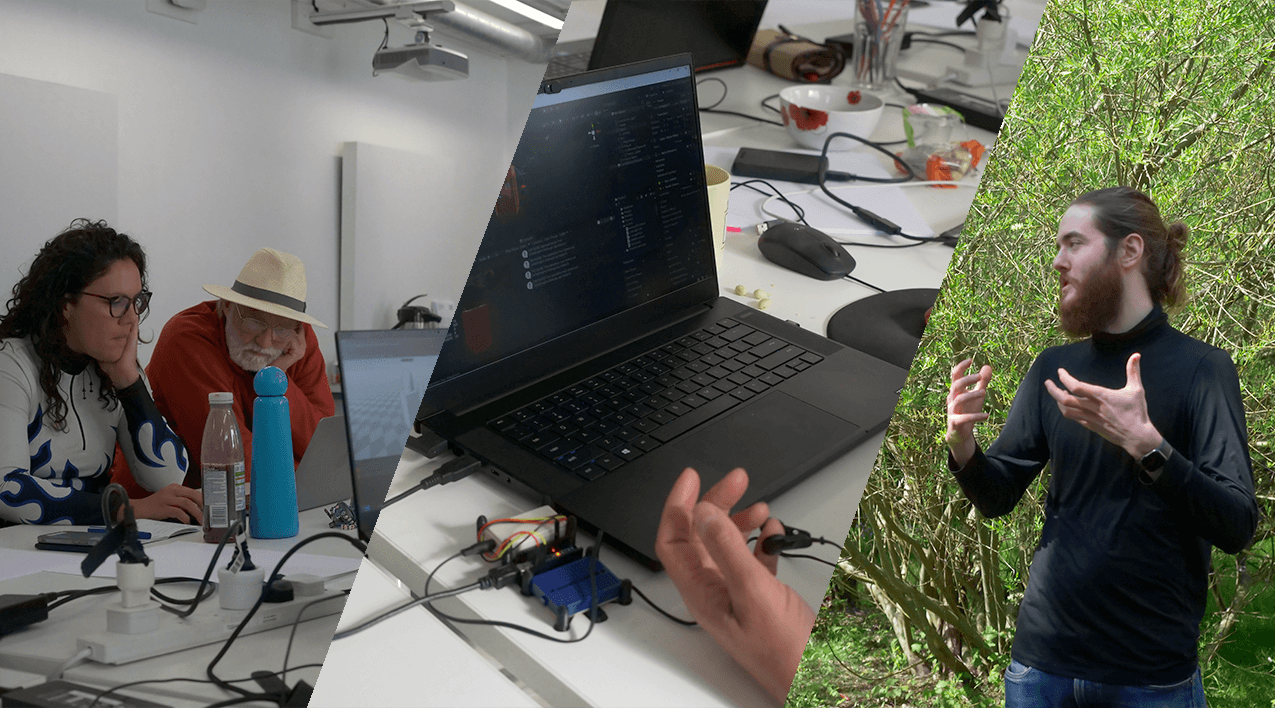
\includegraphics[width=1\linewidth]{02-review/chapter-fig.png}
    \captionsetup{labelformat=empty}
    \caption[\autoref*{sec: review}'s page-figure: We AR in MoMA (from \citeauthor{veenhof2010}, \citeyear{veenhof2010}), Microsoft Hololens 2 in use by the U.S. Army (from \citeauthor{microsoft2021}, \citeyear{microsoft2021}), Project North Star (own photograph)]{}
\end{figure}

\clearpage
% --------------------------------------------------------------------------- %
\section{Summary}\label{sec: review-summary}
This review takes a retrospective view at the history of \gls{ar} technologies. In laying clear the origination of these technologies within predominantly visual fields of research, it allows for a critique of preconceived notions about the definitions of what \gls{ar} is, and the boundaries of how it is used today. The review outlines the contemporary forms, sensory display techniques, and methods taken to mediate our reality with virtual processes. In sketching out this wide variety of possible arising interactions, I make clear the benefit of considering \gls{ar} as a medium for expressive computational artwork, namely in its inherent ability to approach technology from a creative and inclusive perspective (not just from the perspective of viewing \gls{ar} as a visual overlay tool). I then touch on examples of \gls{ar} art that make much more creative use of the materiality of \gls{ar} in this way.



% --------------------------------------------------------------------------- %
\section{History of AR}\label{sec: ar-history}
\begin{wrapfigure}{r}{0.45\textwidth}
    \vspace{-\intextsep}
    \hfill
    \begin{minipage}{0.95\linewidth}
        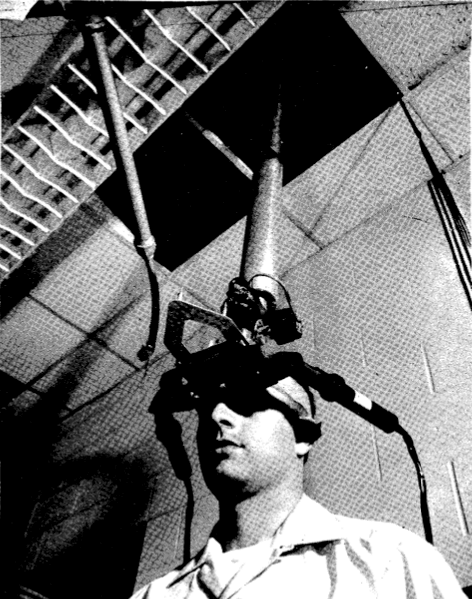
\includegraphics[width=\linewidth]{02-review/sutherland68_2.png}
        \captionsetup{justification=justified}
        \caption{`Head-Mounted Three Dimensional Display' with `The Sword of Damocles' ceiling mounted head tracking device \citep[in][]{sutherland1968}}\label{fig: sutherlandsword}
    \end{minipage}
\end{wrapfigure}
The earliest conceptions of what we would today call \gls{ar} began their development in 1965 with Ivan Sutherland's `Ultimate Display' \citeyearpar{sutherland1965}. Sutherland's project, which was funded by the U.S. \gls{darpa}, involved hypothesising and developing a computer interface that could serve `as many senses as possible'. He speculated that this interface could `serve as a looking-glass into the mathematical wonderland constructed in computer memory'. By \citeyear{sutherland1968}, Sutherland had constructed what he called a `head-mounted three dimensional display', with a which was affixed to the ceiling of his lab with mechanical tracking arm that measured the position and orientation of the display in the room, called `The Sword of Damocles' (see \autoref{fig: sutherlandsword}). The head-mounted display provided per-eye visual displays via reflections from mini-\gls{crt} monitors, whose content was updated in real-time, dependent on the tracked pose of the head. This resulted in the three-dimensional (visual) perception of a hybridised real and virtual space.

Over the course of the proceeding thirty years, most display (visual, audio and haptic) technologies gained higher resolutions, whilst becoming ever more miniaturised, propelled by the general movement towards ubiquitous and wearable computing. In 1992, \gls{ar} was officially defined by Boeing engineers Thomas Caudell and David Mizell, as a technology that could be used to `augment the visual field of the user with information' \citeyearpar{caudell1992}. Their prototype device featured display and tracking technologies that built on the work of Sutherland. The purpose of the Caudell and Mizell's device was to increase manufacture workers' efficiency through overlay of graphical wire-frame instructions. Their device operated by tracking elements of the users environment and body, processing these in real-time, and then overlaying these instructions via a PrivateEye \footnote{\url{https://billbuxton.com/Private_Eye_Brochure.pdf}} in the appropriate places dependent on the manufacturing process, through a \gls{hud} called the `HUDset'. The \glshyperlink[HUDset]{hud}, commonly referred to today as a \gls{hmd} operated by updating the displays output in real-time dependent on the position and orientation (pose) of the participant. This had the effect of the graphical overlay seeming `fixed', or what is referred to now as `registered' or `aligned', on top of a specific point in the real world. For Caudell and Mizell, this display and tracking solution is what leads to the `technology' of \gls{ar} being possible, and for them, it is what enables the context-aware instructional overlay of their application.

\begin{figure}
    \centering
    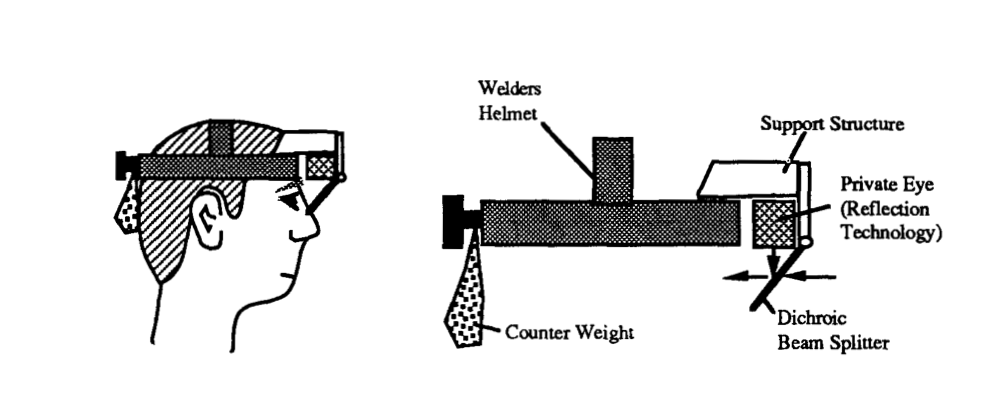
\includegraphics[width=0.75\linewidth]{02-review/caudell92_1.png}
    \captionsetup{justification=centering,margin=1.5cm}
    \caption{Diagram of a `HUDset' using the PrivateEye \citep[in][]{caudell1992}}\label{fig: caudellprivateeye}
\end{figure}

Shortly after this original definition, Milgram and Kishino conceptualised the `Reality-Virtuality Continuum \citeyearpar{milgram1994}, which aimed to consolidate similar efforts across disciplines that were aiming to augment or virtualise `reality'. The continuum (see \autoref{fig: milgramcontinuum}) defines two outer bounds of `Real Environment' on the left (which exist as physical and tangible matter), and `Virtual Environment' on the right (that exist solely as digital bits), and everything within was to be classed as \glsfirst{mr}. Within \gls{mr}, use-cases closer to the `Real' were regarded as \gls{ar}, and use-cases closer to the `Virtual', were regarded as `Augmented Virtuality' (AV). In separating these \gls{mr} use-cases from the tele-robotics field of \gls{vr} and \glspl{ve}, they proposed a clear framework for classifying works. Since both \gls{ar} and AV make use of augmenting `by means of real objects' in today's use cases, (e.g. by tracking and parametrising hand gestures, or tracking and generating spatial maps of the real environment), the difference between \gls{ar} and AV in this definition, problematically, becomes the `primary world' in which objects are are doing the augmenting. Indeed, Milgram and Kishino make note of the possibility of this in their paper: 

\begin{figure}[ht]
    \centering
    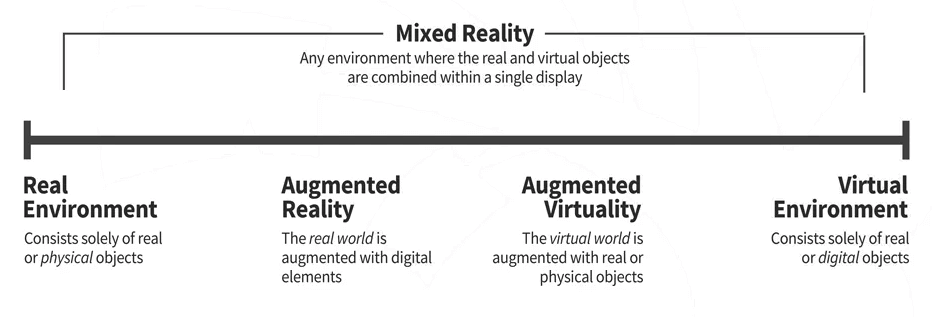
\includegraphics[width=\linewidth]{02-review/tremosa2022.png}
    \captionsetup{justification=centering,margin=1.5cm}
    \caption{Adaptation of the `Reality - Virtuality Continuum' by \citeauthor{milgram1994} \citep[in][]{tremosa2022}}\label{fig: milgramcontinuum}
\end{figure}

`Of course, as technology progresses, it may eventually become less straightforward to perceive whether the primary world being experienced is in fact predominantly `real' or predominantly `virtual', which may ultimately weaken the case for use of both \gls{ar} and AV terms'

They further specify that, despite this is the case, it should not affect the validity of the more general \gls{mr} term to cover the `grey area' in the centre of the virtuality continuum, and also offer the term `Hybrid Reality' for displays that blend \gls{ar} and AV compositely. Today, the term \gls{mr} is seen seldom apart from its use within Microsoft's toolkit, and `Hybrid Reality' even less so. Therefore, as previously mentioned, due to the rapid evolution of these technologies, the present thesis makes no distinction between Mixed, Hybrid, and Augmented Reality.

In \citeyear{azuma1997}, Azuma et al. proposed a specification for the definition of an \gls{ar} system, and surveyed the five years of \gls{ar} research since Caudell and Mizell's original definition. In order to avoid limiting \gls{ar} to specific technologies, they define \gls{ar} as a `system' that follows three characteristics: 

\begin{itemize}
    \item Combines real and virtual
    \item Interactive in real time
    \item Registered in 3-D
\end{itemize}

In this project, also funded by \gls{darpa}, Azuma distinguishes between optical and video based approaches to \gls{ar} and while both of these methods can and had been realised (when speaking strictly of visual display of information) via \gls{hmd} technologies, Azuma makes further room in the definition for monitor based approaches too, allowing the definition to be broad enough to encompass a variety of \gls{ar} use cases, methods and processes. Not soon after, Azuma et al., classify three categories of `display': head worn, handheld and projective. For this reason, as well as the specification of three precise characteristics, Azuma's definition of \gls{ar} has become widespread. 

These early definitions and conceptions of \gls{ar} were typically built upon with applications involving display and tracking technology that resulted in the \textbf{visual overlay and alignment} of \textbf{virtual graphics} onto our \textbf{real world environment}. Whilst this view of \gls{ar} is followed by the overwhelming majority of historical and contemporary uses of \gls{ar}, it only makes up a small subset of the potential myriad interactions afforded by the technologies that enable \gls{ar}. Sutherland, who arguably catalysed early practical research in this field, viewed this \gls{ar} as a `window' interface, that could serve `as many senses as possible'. Louis Rosenberg, a researcher at the U.S. Air Force Research Lab, another early proponent of \gls{ar}, developed the concept of `Virtual Fixtures' (overlaid sensory information) as a method of reducing the `tax' on our senses induced by an overload of information through the visual sense \citep{rosenberg1993}. Milgram and Kishino, in outlining their taxonomy, recognise that it could serve to alleviate `analogous issues associated with other display modalities`, and cite work from Cohen, who at the time was developing realistic acoustic environment rendering in \gls{ar} \citeyearpar{cohen1993}. They also note the concurrent work in haptic (the various senses of touch) displays for \gls{ar}. 

At odds with the typical overlay approach, wearable computing pioneer Steve Mann coined `Mediated Reality' \citeyearpar{mann1994} as descriptor of a methods used to computationally mediate our own perception, rather than focusing on the overlaying paradigm. His later work terms `All Reality (*R)' which broadens the taxonomy of \gls{ar} with concepts such as as surveillance and privacy \citeyearpar{mann2018}. Azuma et al., also acknowledge that \gls{ar} is not just limited to visual perception or overlaying processes: `\gls{ar} can potentially apply to all senses, including hearing, touch, and smell. Certain \gls{ar} applications also require removing real objects from the perceived environment, in addition to adding virtual objects'. With this in mind, what does the landscape of more contemporary \gls{ar} design look and feel like today?




% --------------------------------------------------------------------------- %
\section{Forms of AR}\label{sec: ar-forms}
\subsection{Head-mounted}\label{sec: ar-forms-hmd}
\begin{figure}
    \centering
    \captionsetup{justification=centering}
    \subcaptionbox{`Head-Mounted Three Dimensional Display' \citep[in][]{sutherland1968}\label{fig: historicalHMDs-sutherland}}[.3\linewidth]{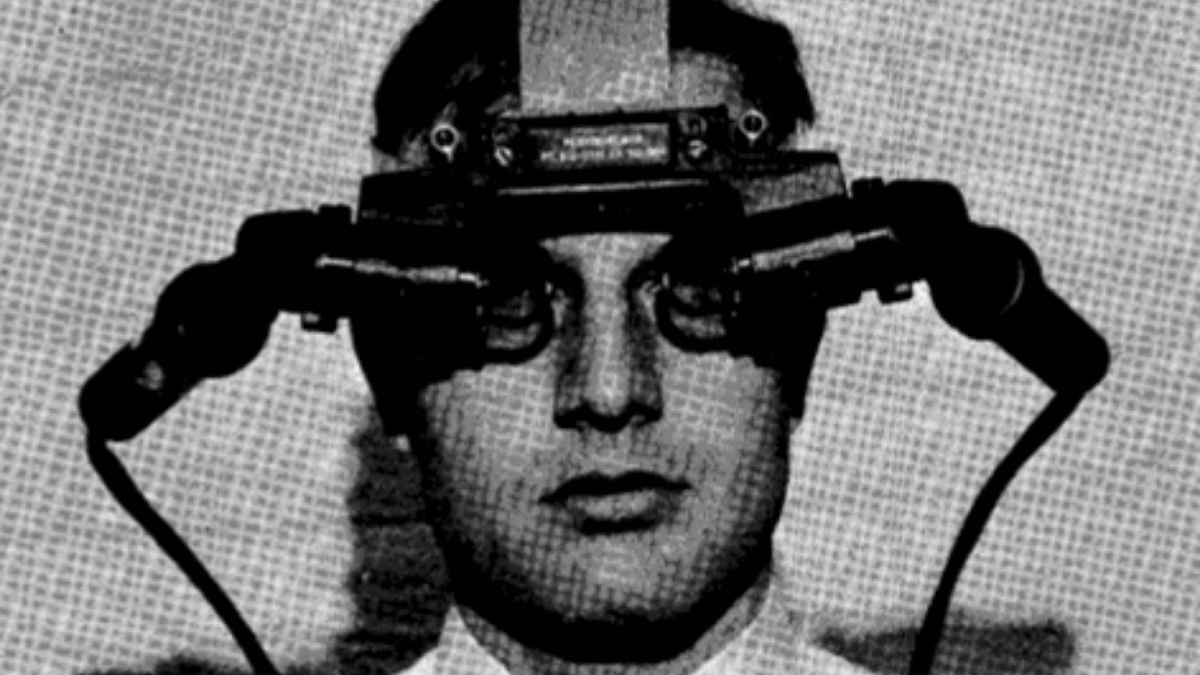
\includegraphics[height=2.5cm]{02-review/sutherland68_1.png}}
    \hfill
    \subcaptionbox{`HUDset' \citep[in][]{caudell1992}\label{fig: historicalHMDs-caudell}}[.3\linewidth]{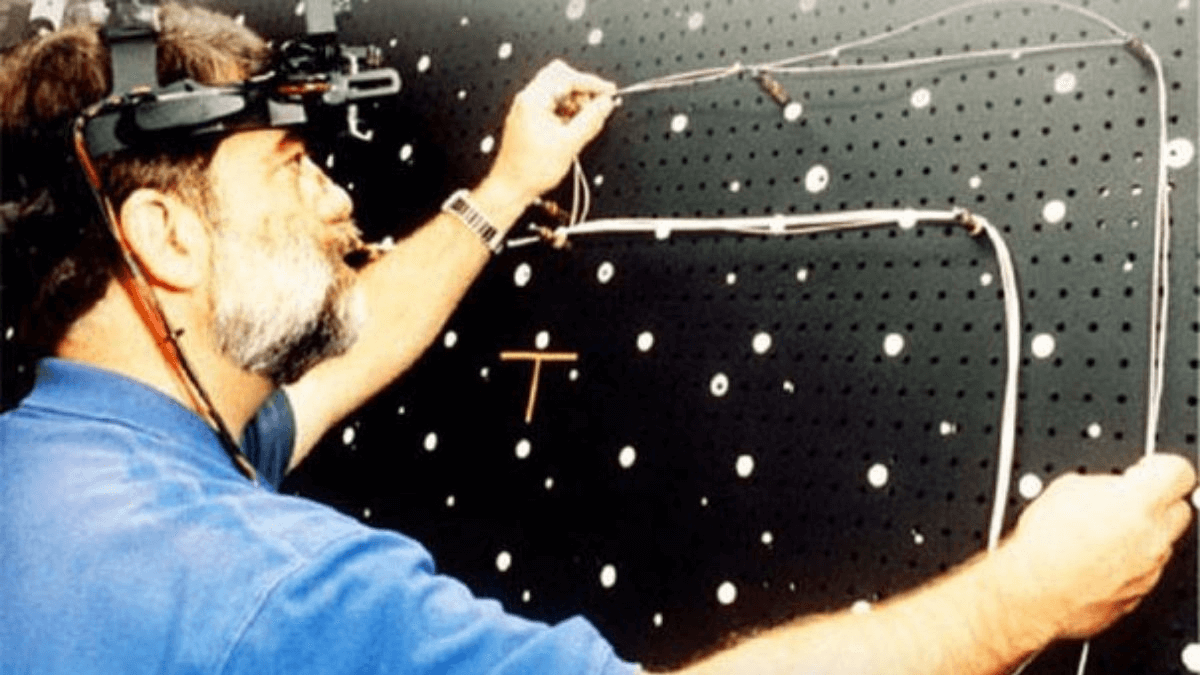
\includegraphics[height=2.5cm]{02-review/caudell92_2.png}}
    \hfill
    \subcaptionbox{`KARMA System' \citep[in][]{feiner1993}\label{fig: historicalHMDs-feiner}}[.3\linewidth]{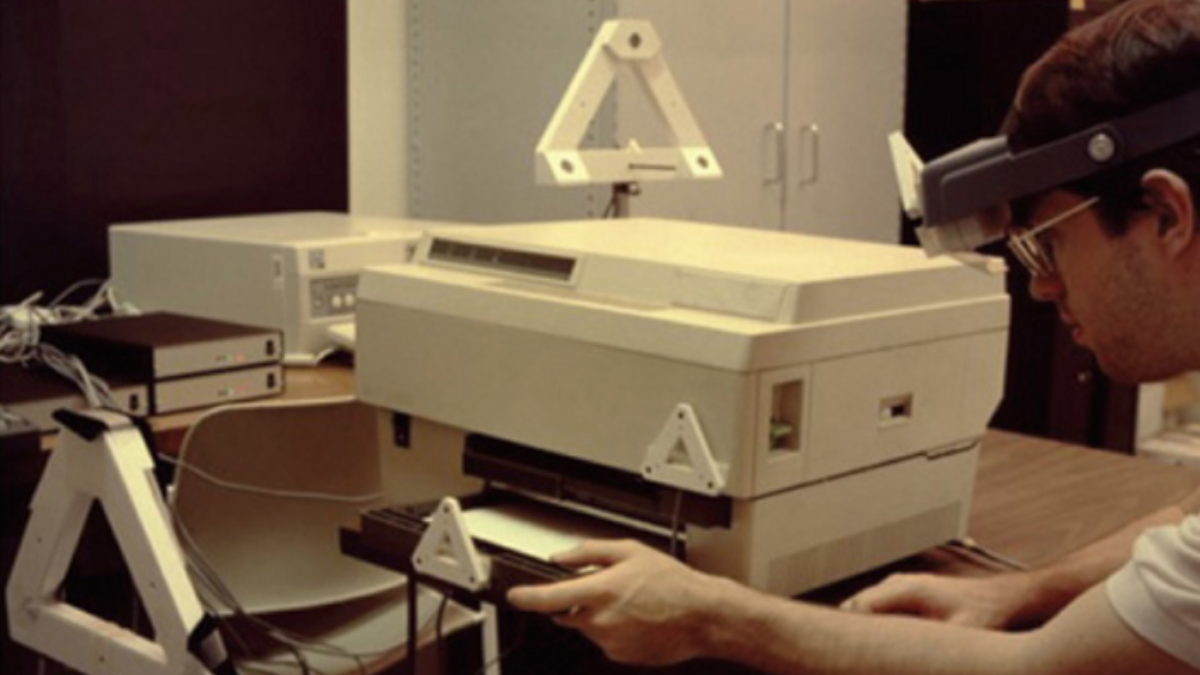
\includegraphics[height=2.5cm]{02-review/feiner93_1.png}}%
    \caption{Augmented Reality Head Mounted Displays in the 20th Century}
    \label{fig: historicalHMDs}
\end{figure}
Successors of \gls{ar} \glsplural{hmd} devised by Sutherland \citeyearpar{sutherland1968}, Caudell and Mizell \citeyearpar{caudell1992}, and Feiner \citeyearpar{feiner1993,feiner1997} exist today commercially within products such as the Microsoft Hololens 2 \footnote{\url{https://www.microsoft.com/en-us/hololens}}, the Magic Leap ML-1 \footnote{\url{https://www.magicleap.com/magic-leap-1}}, and the nReal Light \footnote{\url{https://nreal.ai/product/}}. These devices afford optical see-through capabilities through half-mirror visors and high-resolution displays, and offer stereo audio output. Input is managed mainly by hand-tracked interaction with overlaid visual menus and objects, but is also possible through eye tracking and voice control. The environment is sensed through a combination of \gls{6dof} tracking, and spatial mesh mapping. For most \glsplural{hmd} today, this input and environment processing occurs off-device, on a tethered or wearable computer, or mobile device. These devices tend to be relatively expensive due to the extremely high R\&D costs associated with the field (due to its novelty). Leap Motion's \glshyperlink[open-source]{opensource} \gls{pns} \footnote{\url{https://docs.projectnorthstar.org/}} provides a much cheaper alternative at the trade-off of slightly larger form and lack of integrated computing and audio implementation, but has the highest field-of-view of all four and comparable tracking.

%*[ ]   fix figure
\begin{figure}
    \centering
    \captionsetup{justification=centering}
    \subcaptionbox{Microsoft Hololens 2 \citep[from][]{microsoft2022}\label{fig: contemporaryHMDs-microsoft}}{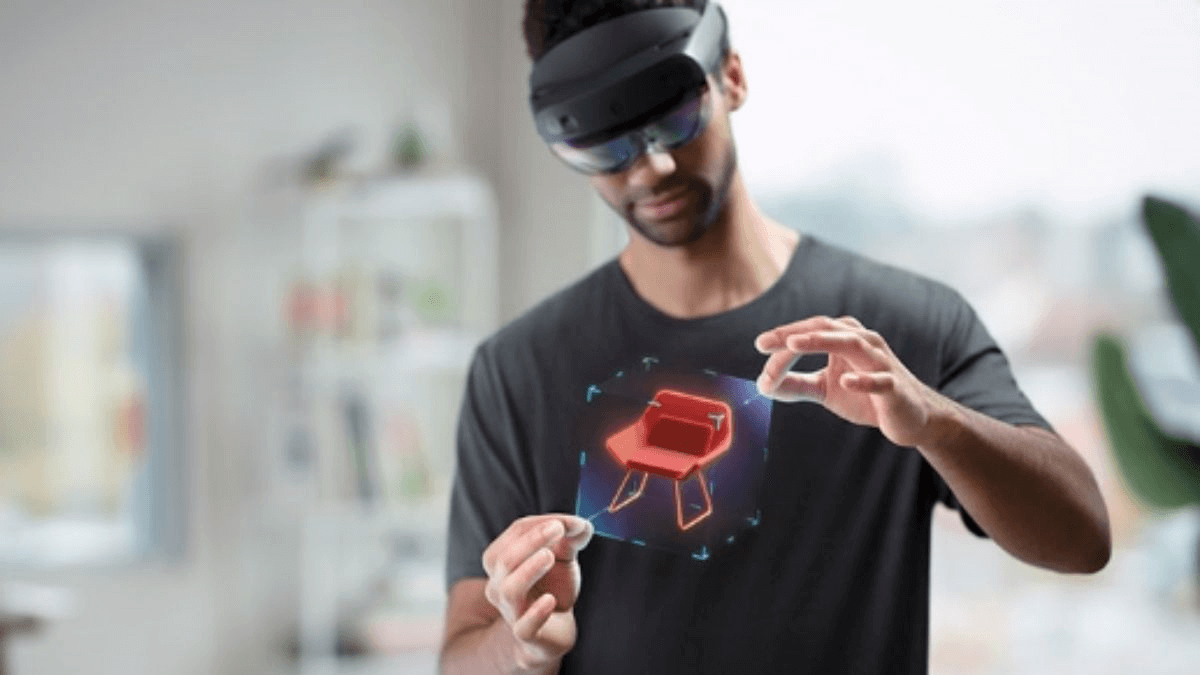
\includegraphics[width=0.45\linewidth]{02-review/hololens.png}}\quad
    \hfill
    \subcaptionbox{Magic Leap ML-1 \citep[from][]{att2019}\label{fig: contemporaryHMDs-magicleap}}{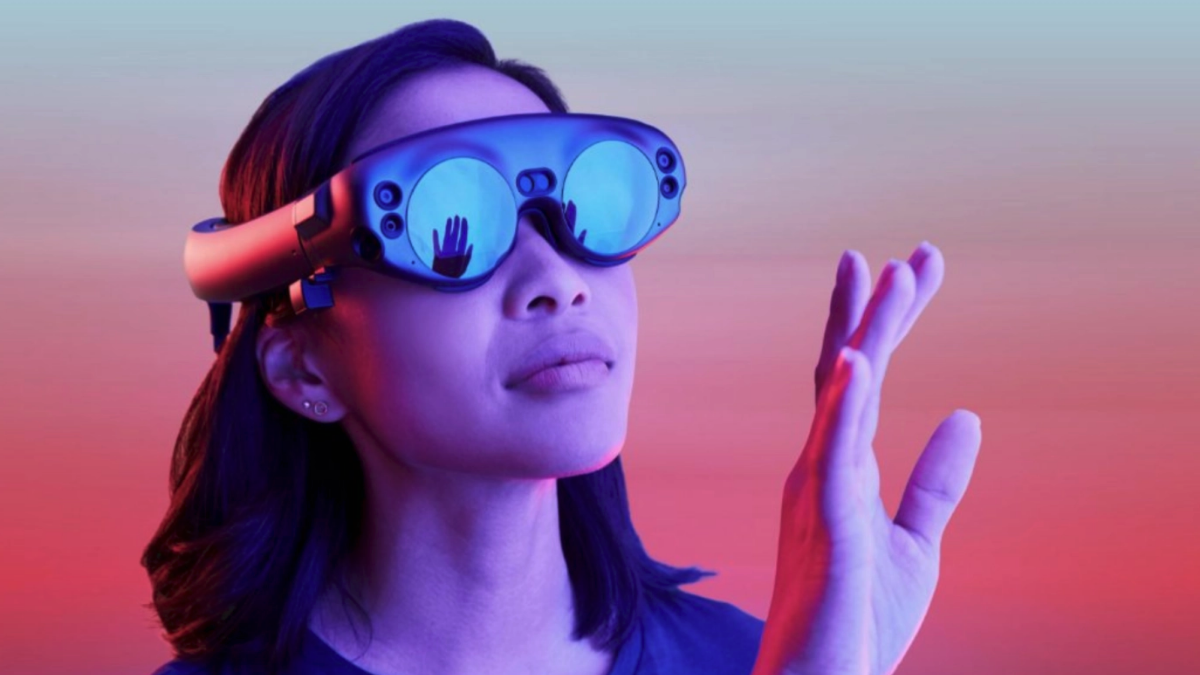
\includegraphics[width=0.45\linewidth]{02-review/magicleap.png}}\\
    \vspace{0.5cm}
    \subcaptionbox{nReal Light \citep[from][]{nreal2020}\label{fig: contemporaryHMDs-nreal}}{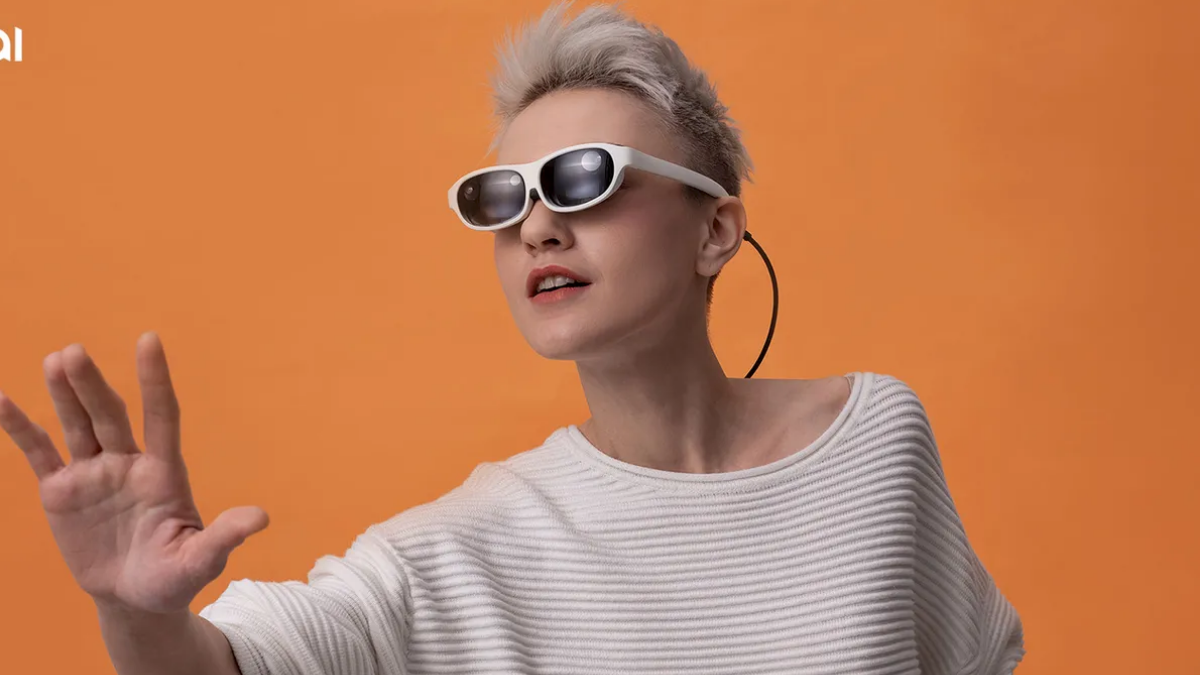
\includegraphics[width=0.45\linewidth]{02-review/nreal.png}}\quad
    \hfill
    \subcaptionbox{Leap Motion Project North Star \citep[in][]{bilbow2022}\label{fig: contemporaryHMDs-northstar}}{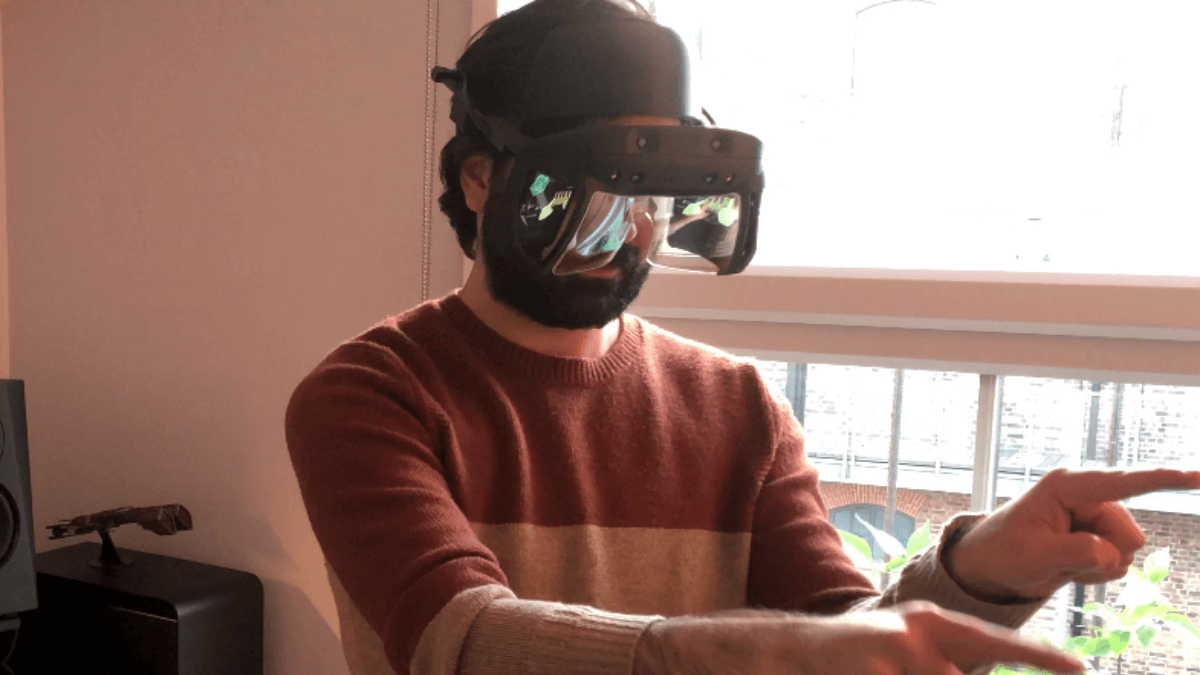
\includegraphics[width=0.45\linewidth]{02-review/northstar.png}}\\
    \caption{Augmented Reality Head Mounted Displays in the 21st Century}
    \label{fig: contemporaryHMDs}
\end{figure}

A device that is head-mounted poses clear benefits to both input and output modalities. For input sensors, being mounted on the head provides them with more accurate tracking from the perspectives of our own senses (organic sensors). Consequently, and as Lindeman and Noma maintain in their classification scheme for \gls{msar}, an important factor for the parity (if desired) of real and virtual output is a consideration of the location along the `stimulus pathway' at which they mix: at the environment, sensory subsystem or computer level \citeyearpar{lindeman2007}. For a device to be head-mounted, allows `mixing' to happen closer to the sensory subsystems, e.g., our eyes, ears, nose and mouth, thus resulting in an experience that is more closely intertwined with our real-time environment stimuli.

\subsection{Handheld}\label{sec: ar-forms-mobile}
Today, anyone who owns a smartphone is carrying an \gls{ar} device in their pocket. This particular genre of \gls{ar} development began in earnest in the mid 2000's and today is the most widely used form of \gls{ar} due to the pervasiveness of smartphones. It builds on the early research and practice of handheld \gls{ar} applications built on cellphones and \glspl{pda} in the late 1990's, and smartphones in the late 2000's, whose increasing variety and accuracy of onboard sensors: cameras, gyroscopes, accelerometers, and \gls{satnav}, provided a convenient all-in-one solutions for developing handheld visual \gls{ar} experiences. 

The limitations of handheld displays are outlined by Bimber and Raskar \citeyearpar[pp. 79-83]{bimber2005}: reduced immersiveness due to the small screen size, compounded by the distance between it and the participant (normally arms length), impaired gestural input due to the need to hold the device; restrictions due to the cameras image quality and less computational power available to effectively register (align) real and virtual objects. As well as these issues, smartphones have developed to be primarily visual devices despite their name, and as such, their ability to deliver high fidelity audio, let alone \gls{aar} mixing is limited due to their distance from the ear. 

Recently, the lack of non-visual \gls{ar} in handheld smartphones has been addressed through the increased adoption of `hearables', a marketing term for small and unobtrusive, wireless earphones. More specifically, two features make these suitable audio solutions for \gls{ar} use; `transparent' hearing modes (see mic-through \citep{lindeman2008}), and integrated \gls{6dof} tracking \footnote{\url{https://www.apple.com/airpods-pro/specs/}}.

\subsection{Projective}\label{sec: ar-forms-proj}
Projection of data into the environment in order to overlay or alter perception of real objects, i.e. mixing virtual and real stimuli at the environment level \citep{lindeman2007}, is perhaps the least adopted of Azuma's categories of \gls{ar}. The property that sets projective \gls{ar} apart from head-mounted and handheld \gls{ar} is its potential to deliver experience to multiple participants within a shared space. Although collaboration is possible through the previous two categories, it requires all participants to engage technology that is affixed to their body (either through wearing or through holding). Projective \gls{ar} alleviates both the burden of physical attachment to a device, and also the expense of procuring a device for each participant. This category of display is typically realised by use of video projectors and speaker arrays. Although the base requirement of registration in three-dimensions between virtual and real (Azuma's third specification), is fulfilled relatively easily compared to head-worn and handheld approaches (more sensor computation and accuracy), 

\subsection{Other Forms}\label{sec: ar-forms-other}
Of course, this categorisation of forms is not exhaustive, and leaves out body worn \gls{ar} systems such as haptic vests, systems that take on more than one form such as the Audiomented Sound System / Parabolic Mirror in Listening Mirrors \citep{chevalier2020}, and sonically tangible virtual objects \citep{schraffenberger2015}. I will expand on these cases in \autoref{sec: discussion-patterns-instrument}, where I lay out a design pattern for considering wearable, tangible, and situated \gls{ar} instruments.



% --------------------------------------------------------------------------- %
\section{Sensory Display in AR}\label{sec: ar-sensory}
Within these common forms of \gls{ar} technology, one could split the various technological processes that occur into input, process, output (the general IPO model found in software engineering), in \gls{ar} this is often labelled: tracking, process, display. Tracking, as mentioned is often through hand gesture, body position and orientation and voice activation. Display is managed in the majority of cases through screens. The present section outlines various other sensory displays that have the potential of creating more immersive tools of expression.

\subsection{Visual Sense}\label{sec: ar-sensory-visual}
It is poignant to mention that until that last 20 years or so, sensory sciences, and as a result, technological displays of information, were focused on the visual, with the auditory following behind, and then the touch, smell and taste senses. In cross-modality psychology research, this ocularcentrism (the perceptual and epistemological bias ranking vision over other senses) is normally explained by a `textbook' explanation: `the idea that vision is the most important modality is supported by numerous studies demonstrating visual dominance.' Fabian Hutmacher argues that ocularcentrism can be critiqued through the lenses of \citeyearpar{hutmacher2019}: 

\begin{itemize}
    \item A methodological-structural explanation: `Research on vision is often easier than research on other modalities and that this is the result of an initial bias toward vision that reinforces itself.'
    \item A cultural explanation: `The dominance of the visual is not a historical constant, but rather a result of the way (Western) societies are designed.'
\end{itemize}

However, \gls{ar} is still typically realised in the form of graphical overlay, and as such, the forms which we find ourselves interacting with are predominantly based around screens and other forms of visual display \citep{dey2018}. These are often split into optical and video see-through methods of display. The former employs semi-reflective half-mirrors to combine the reflection of close-by screen with the natural pass-through of the real world; the latter uses the feed of cameras to completely occlude the participant's vision, and performs \gls{ar} processes on top of the camera feed. There are advantages and disadvantages to both methods, outlined in \citep{rolland2000}. Head-mounted systems tend towards optical see-through, whereas most handheld \gls{ar} (smartphones) are exhibit video see-through \gls{ar}.

\subsection{Auditory Sense}\label{sec: ar-sensory-auditory}
The second most developed-for sense in \gls{ar} is the auditory system, borrowing from a rich history of spatial audio techniques such as exploiting \glspl{hrtf} for binaural audio playback and realistic audio localisation \citep{blauert1969,blauert1996}. Within the field of \gls{aar}, as previously mentioned, `hearables' with `transparency hearing' modes offer the auditory equivalent of video see-through (coined mic-through \citep{lindeman2008}), where the occluded outside world is captured through a microphone, on top of which virtual sounds can be processed. Also outlined by Lindeman and Noma is the use of bone conduction headphones to offer a mediated perception of sound environments without the need to occlude the participants ears (coined hear-through), which could be considered equivalent to optical see-through. Moving into the environment, there are a myriad spatial audio techniques that could be used within \gls{ar}, delivered by speaker arrays such as those found in wave-field synthesis \citep{berkhout1993} and ambisonic beam-forming practices \citep{sharma2018,mcarthur2019}.

\subsection{Haptic Sense}\label{sec: ar-sensory-haptic}
Due to the prevalence of hand-tracking technologies in the interaction with head-mounted \gls{ar} applications, one might assume that being able to actually \textit{feel} the virtual objects that are placed in \gls{ar} would be one of the most important and developed concepts in \gls{ar}. However, much of the early research in \gls{ar} placed importance around overlaying instructions, rather than interactive objects. Hence, the haptic feedback of touching \gls{ar} objects is relatively under-explored compared to the common issues which affected early and (funded) research - accurate registration of real and virtual processes; and higher visual fidelity. In most cases, it was deemed enough to \textit{see} the effect that ones hands or body position had on the \gls{ar} object or scene respectively. Today, there exist numerous technologies that could provide computationally mediated haptic perception in \gls{ar}, for example through vibrotactile feedback or electrical muscle stimulation \citep{lopes2018}, and more recently ultrasound mid-air haptic sensations \cite{ablart2019}.

\subsection{The Chemical Senses}\label{sec: ar-sensory-chemical}
\begin{wrapfigure}{r}{0.45\textwidth}
    \vspace{-\intextsep}
    \hfill
    \begin{minipage}{0.95\linewidth}
            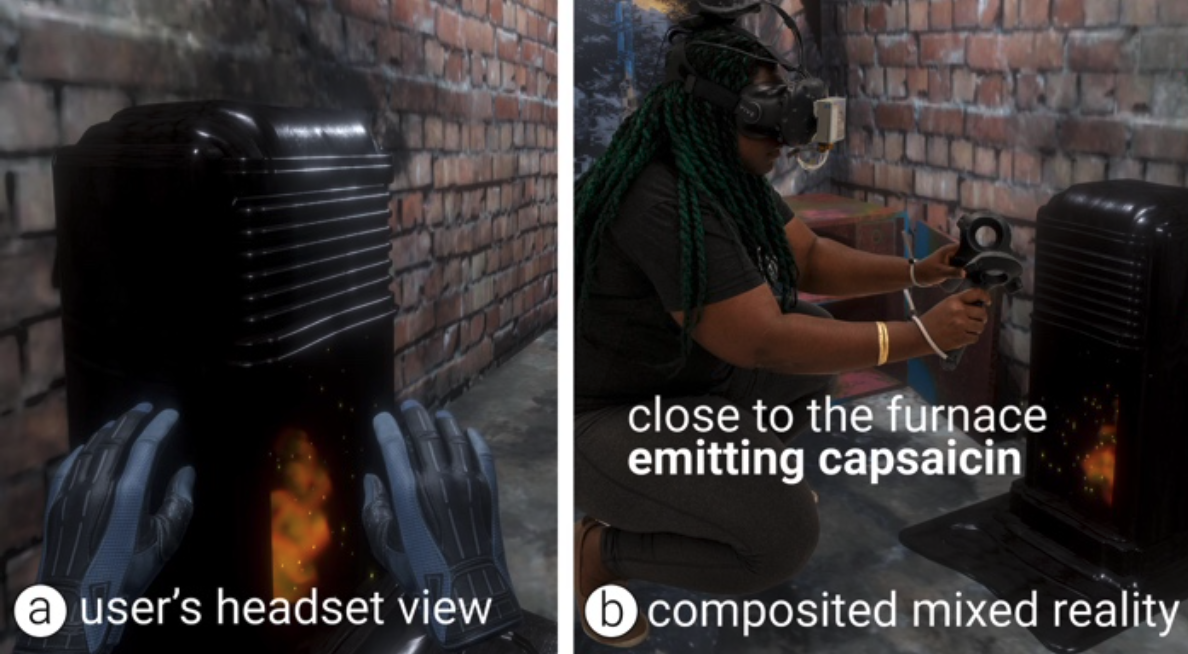
\includegraphics[width=\linewidth]{02-review/brooks2020.png}
            \captionsetup{justification=justified}
            \caption{A participant shown in (a) VR and (b) artificial composite mixed reality. The participant is being warmed by a furnace, as the device atomizes a cayenne pepper tincture (capsaicin) to create a warming sensation in their nose \citep[in][]{brooks2020}}\label{fig: brooks2020}
    \end{minipage}
\end{wrapfigure}
Whereas auditory and haptic sensations have been developed in \gls{ar}, the chemical senses (smell and taste) have received far less exploration. Visual, auditory, and touch information can be believably recreated with technology through analog to digital conversion of electromagnetic radiation (light) and mechanical wave transmission (sound and touch). Conversely, smells and tastes contain organic information, the sensors (and thus analog-digital conversion) for which have not been invented yet. As such, the closest we can get to receiving chemical sensory data is through computationally activated rather than computationally mediated displays: scent emitters \citep{maggioni2019}, and taste patches for example. Accordingly, in order to mediate the sense of taste, creative methods of sensory illusion have often been employed, e.g. Narumi et al. demonstrating that the sense of flavour can be mediated via visual overlay in \gls{ar} \citep{narumi2011}. The sense of temperature has also been mediated through cross-modal sensory illusion (see \autoref{fig: brooks2020}) exploiting the trigeminal nerve in the nose, \citeauthor{brooks2020} demonstrate that users in \gls{vr} can be made to feel warmer or colder based on the relative amounts of capsaicin or eucalyptus emitted near the nose \citeyearpar{brooks2020}.



% --------------------------------------------------------------------------- %
\section{Processes in AR}\label{sec: ar-process}
Additive layering of virtual content onto our real environment is by far the most typical of processes experienced in \gls{ar}. However, it is only one of the potential methods of interaction between virtual and real components. In navigating this issue, the present thesis aligns its conception of \gls{ar} closely with the definition of \gls{ar} by Chevalier and Kiefer \citeyearpar{chevalier2020}: `real-time computationally mediated perception', which fulfils Azuma's three characteristics of \gls{ar} systems, but is not as exclusionary as Caudell and Mizell's original definition: a technology used to  `augment the visual field of the user with information'. Investigating the existing relationships between real and virtual components of \gls{ar} systems, Schraffenberger outlines at least five `relationships' and five `subforms' of \gls{ar} (see \autoref{table:schraffenbergertaxonomy}). This taxonomy \citeyearpar[pp. 80-130]{schraffenberger2018} provides an ideal starting point for those designing \gls{ar} systems interested in creating embodied experiences that challenge the typicality of basic visual-overlay \gls{ar}. Furthermore, Mann expands the `Reality - Virtuality Continuum' \citep{milgram1994} into the `All Reality Continuum', integrating further dimensions such as `Metaveillance', `Kineveillance' and `Phenomenality', such a standpoint not only `anticipates the need for an ethically aligned reality' \citeyearpar{mann2018}, but demonstrates the multifaceted nature of \gls{ar} to afford experiences of ourselves, others, and environments computationally mediated by more than just additive informational overlays.

\begin{table}[ht]
    \centering
    \begin{tabular}{ l l }
        \toprule
        Relationship        & Description                       \\
        \midrule
        Coexistence         & Unrelated                         \\
        Presence            & Spatially Related                 \\
        Information         & Content-Based Relationship        \\
        Physical            & Affect Each Other                 \\
        Behavioural         & Sense and React to Each Other     \\
        \midrule
        \midrule
        Subform             & Description                       \\
        \midrule
        Extended Reality    & The Virtual Supplements the Real  \\
        Diminished Reality  & The Virtual Removes the Real      \\
        Altered Reality     & The Virtual Transforms the Real   \\
        Hybrid Reality      & The Virtual Completes the Real    \\
        Extended Perception & Translating the Imperceptible     \\
        \bottomrule
    \end{tabular}
    \captionsetup{justification=centering,margin=1.5cm}
    \caption{Taxonomy of relationships and emergent AR subforms \citep[in][]{schraffenberger2018}}\label{table:schraffenbergertaxonomy}
\end{table}

In particular, `diminished reality', aims to \textit{remove} real objects in our environment. When explored in the visual sense, this approach uses computer vision and content-aware substitution to remove a section or object of the real-world environment through camera sensors. Noise cancelling potentially offers an auditory diminished reality, but due to the fact that sound is propagated via mechanical waves, our sense of sound is closely intertwined with physically feelings of vibration, which are much harder to remove \citep{mori2017}. Further examples of sound-driven but cross-modal techniques are outlined in \citep{walther-hansen2020}.

\begin{wrapfigure}{l}{0.45\textwidth}
    \vspace{-\intextsep}
    \begin{minipage}{0.95\linewidth}
        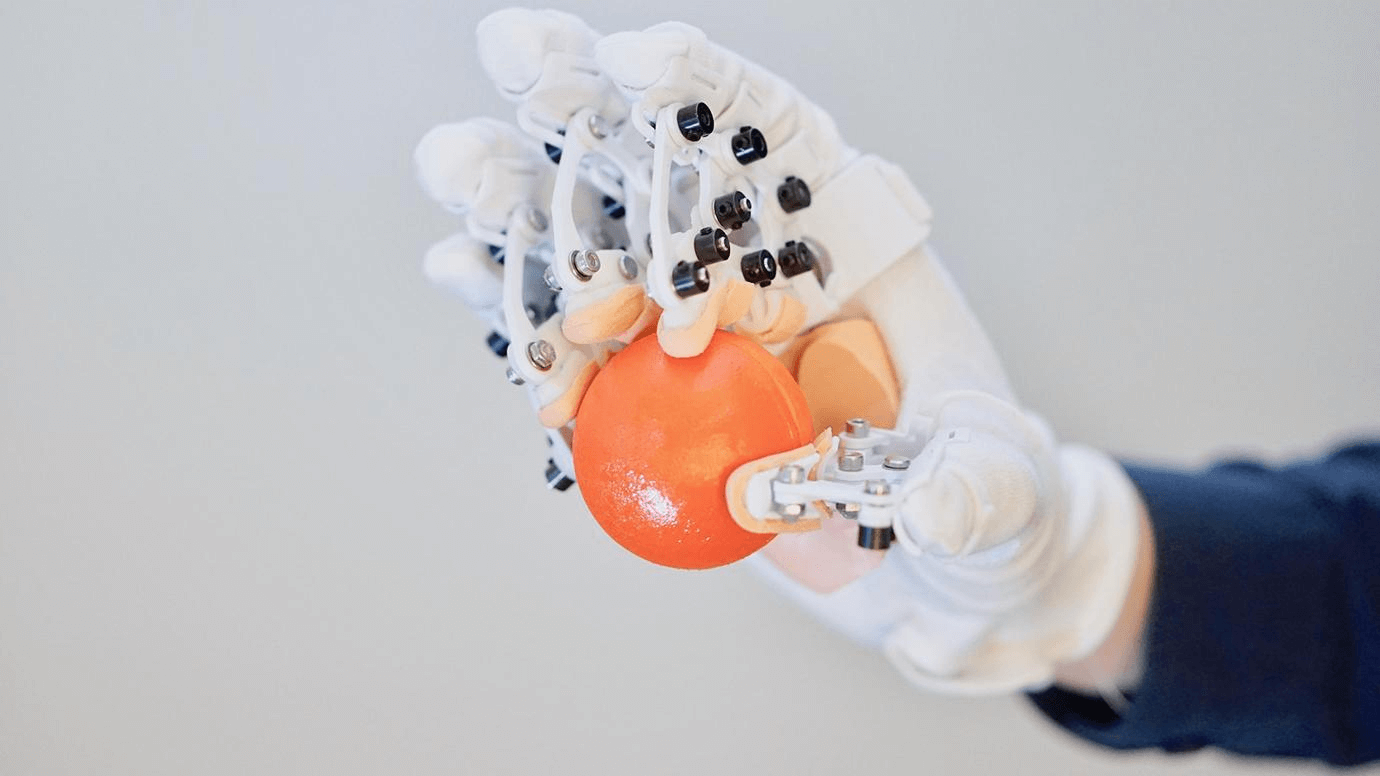
\includegraphics[width=\linewidth]{02-review/nishida20_1.png}
        \captionsetup{justification=justified}
        \caption{`HandMorph' offers altered touch perception by reducing hand affordances \citep[in][]{nishida2020}}\label{fig: handmorph}
    \end{minipage}
    \hfill
\end{wrapfigure}
`Altered reality' has the potential to provide new and otherwise inaccessible sensory and perceptual experience Schraffenberger describes that this is possible through virtual components altering the perception of real components in an \gls{ar} system. Mann outlines a myriad examples of altered visual percepts \citeyearpar{mann1994}, from giants eyes, to `slow' glasses. More recently, Nishida et al. have experimented with `egocentric smaller-person experience' through use of a video see-through \gls{ar} headset, in which unlike typical \gls{ar}, the cameras are mounted at waist height, rather than on the \gls{hmd} \citeyearpar{nishida2019}. This afforded participants a difference in real-time visual perception, and resulted in them generally feeling smaller and behaving more like a child. In tandem with this altered visual perception, they propose a modified robotic glove `HandMorph' \citeyearpar{nishida2020} that alters sensations of touch through reduced finger and overall grip size. 

\begin{wrapfigure}{r}{0.45\textwidth}
    \hfill
    \begin{minipage}{0.95\linewidth}
        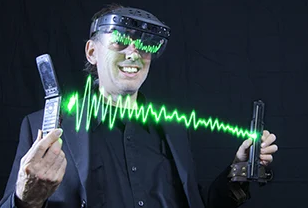
\includegraphics[width=\linewidth]{02-review/mann18_1.png}
        \captionsetup{justification=justified}
        \caption{`Sequential Wave Imprinting Machine' allows visualisation of radio waves in AR \citep[in][]{mann2018a}}\label{fig: mann_swim}
    \end{minipage}
\end{wrapfigure}
In a similar vein, `extended perception' revolves around the potential to provide \textit{more} senses, or the sensing of stimuli outside of the range of our sensory systems. Bees for example have a visual system that extends far further into the ultraviolet range of EM radiation than our own eyes allow us; dogs hear much higher frequencies our ears allow us (thank goodness); and sharks can smell one part blood in a million parts water. These fun facts demonstrate vast differences in sensory acuity between species; but did you know that some shark have a constellation of pores \footnote{\url{https://www.sharktrust.org/shark-senses}} along the lateral side of their bodies that allows them to perceive minute pressure changes in water? This enables them to create a `pressure map' of their surroundings through active body movement. Modern technology could endow us with similar and myriad extended perceptions of our environment and its stimuli; Mann has experimented with making representations of radio waves translated down to the sensory range of our own eyes \citeyearpar{mann2018a}.

This section demonstrates the multitude of potential experiences that \gls{ar} affords beyond mere visual information layering, next, I will examine the usage of \gls{ar} in the arts, as a medium or tool for creating immersive aesthetic experiences, and demonstrate how this contributes towards a more holistic understanding of \gls{ar} as a technology. 



% --------------------------------------------------------------------------- %
\section{AR in the Arts}\label{sec: ar-arts}
The present chapter has outlined the origins of \gls{ar} technology in funding from the U.S. \gls{mic}. This is in the hope of making clear that the challenge faced by \gls{ar}'s co-option in the arts is not just one that is at odds with its origin technologically and functionally, but also ethically, morally, and socio-culturally. The dominance of the visual sense, and of the process of overlaying, is a direct consequence of the importance of these approaches in the military and industry applications of \gls{ar} (and more generally, digital technology) within the the capitalistic and colonial pursuits of . Let us not forget that the first explicitly defined `\gls{ar}' application was as a tool to increase worker efficiency \citep{caudell1992}, perhaps for safety, perhaps for quality assurance, but most likely for streamlining the workforce and increasing profits. Around the same time, \gls{hud} technology was being used by the military to increase the deadliness of US fighter pilots by offering the tactical advantage of visual and auditory overlay of target locations \citep{wanstall1989}. 

One might be mistaken for thinking that this was just an opening chapter in the story of \gls{ar}, but unfortunately for those of us who oppose the regressive neo-colonial and capitalist elements of global \glspl{mic}, \gls{ar} technology is still very much in receipt of advancement from these same industries. In 2018 the U.S. Army was looking to award a contract worth over \$500 million USD to an \gls{ar} headset manufacturer for the production of 100,000 headsets for their soldiers to `increase lethality by enhancing the ability to detect, decide and engage before the enemy' \citep{brustein2018}. Both Magic Leap and Microsoft bid on the contract, with Microsoft ultimately being awarded it. Though this commentary is at risk of lacking nuance, and the above outlined example may read as being a consequence of `technological progress', I hope to impart that this is the intended direction of \gls{ar} funding, rather than an accident. This can serve to empower those who aim to implement and appropriate the same technologies creatively. This is not a new story, rather a relationship as old

How, as artists and musicians opposed to the pursuit for what can only be described as techno-dystopian `super soldiers', can we navigate this space morally and co-opt these tools for positive social change -- is it even possible? Moving forwards I would like to suggest three areas from which we may be able to think about \gls{ar} differently. These stem from the categorisation by \citep{azuma1997} of \gls{ar} but aim to go beyond the technological and functional, which may be tinged with values and predispositions towards military and industrial applications. This is in order to engage with these three characteristics from a digital arts and humanities perspective:

Azuma et al. specify:
\begin{itemize}
    \item \gls{ar} combines real and virtual
    \item \gls{ar} is interactive in real time
    \item \gls{ar} is registered in 3-D
\end{itemize}
We ask:
\begin{itemize}
    \item How does this combination result in \textbf{material} that makes up an \gls{ar} experience?
    \item How do interactive \gls{ar} experiences engage our sense of \textbf{embodiment}?
    \item How can we describe the hybridity of registered \textbf{space} in \gls{ar} experiences?
\end{itemize}

Agreeing that \gls{ar} can be used as a medium for the composition of computational art, provides the starting point from which to answer these questions. As Papagiannis highlights, we ought to develop an understanding of the `capacities of the technology and its constraints, to exploit the technology to artistic use by envisioning novel applications and approaches, and developing new aesthetics and conventions beyond previous traditional forms' \citeyearpar{papagiannis2017}. If visual overlay \gls{ar} has been used as `a viewing instrument to bring into focus forces invisible to the naked or unknowing eye, and make them visible in the public sphere.' \citep{thiel2011}, what emergent properties might applications rising out from multisensory approaches to design afford? What are the futures of digital musical instruments, whose designers opt to use this medium? 

Among other creative fields, computational art has already seen some nascent implementation of \gls{ar} as a medium. Computational art, the use of computational programming or software as a tool, performance aid, medium or collaborator to create art or artistic works, is currently witnessing the adoption of new and exciting technologies such as trained machine learning algorithms, increasingly immersive displays and large-scale networked experiences. These implementations of technology within the creation of artworks leads to a greater understanding of the materiality of these technologies, and perhaps greater understanding of the self and others. In this section, I draw attention to contemporary examples of artworks that demonstrate the modes of sensory engagement, aesthetic experience, collaborative expression, and activism that \gls{ar} specifically affords these artists that are willing to exploit its use as a medium.

\subsection{Sensory Engagement}\label{sec: ar-arts-sensory}
Computational art has seen the use of \gls{ar} as a medium since the early 1980's. in 2008, Grasset et al. presented case studies of \gls{ar} art exhibitions, with the conclusion that for effective design of artworks, specific importance should be placed on the relationship \textit{between} real and virtual components \citeyearpar{grasset2008}. These relationships have come to describe a matrix of possibilities between senses and mediating processes, e.g. altered hearing, extended smell, diminished sight. Papagiannis has drawn attention to this broader multisensory view of \gls{ar} in attempting to understand an aesthetic for \gls{ar} applications, `AR is beginning to expand in new ways, beyond visual frames and into the full human sensorium' \citeyearpar{papagiannis2014}. In 2015, the Tate Sensorium multisensory art exhibition used novel mid-air haptic devices to augment visual art \citep{vi2017a}. The results of the included study found that more congruent multisensory experiences lead to audiences finding artwork more emotionally engaging. If more congruent multisensory experiences of art lead to more emotional engagement, and \gls{ar} has the potential to mediate multiple senses in rich and provocative ways, surely this makes it an ideal medium for such works. 

\begin{figure}[ht]
    \centering
    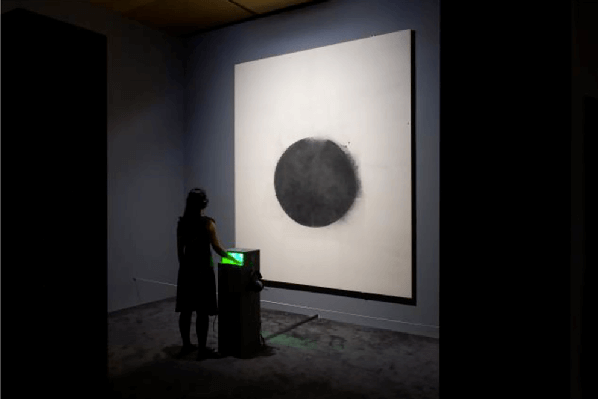
\includegraphics[width=.75\linewidth]{02-review/vi17_1.png}
    \captionsetup{justification=centering,margin=1.5cm}
    \caption{Tate Sensorium multisensory ARt providing audio and haptic augmentation \citep[in][]{vi2017a}}\label{fig: tate}
\end{figure}

\subsection{Aesthetic Experience}\label{sec: ar-arts-aesthetics}
Chevalier and Kiefer highlight the nascent use of newer \gls{ar} technologies by artists \citeyearpar{chevalier2020}. They argue that \gls{ar} has far more potential for creative exploration, and that it is a medium for creating `new nuanced and fine-grained emergent aesthetic experiences' and as previously mentioned, necessarily define \gls{ar} as `real-time computationally mediated perception' in order to be inclusive of a multisensory approach to design. 

The installation `Concrete Storm'\footnote{\url{https://www.studiodrift.com/concrete-storm-microsoft}} by artists Gordijn and Nauta demonstrates the ability for \gls{ar} to afford novel experiences of seemingly immutable and rigid physical objects (short concrete pillars), through the extension and animation of the concrete into larger, shifting and breaking structures. In describing the design of the work, they outline one of the main impetuses of creating the work: `Gordijn says the duo was interested in beginning to investigate the point at which viewers `might let go of trying to distinguish between what is real, what is not' and accept this new mixed world as simply another version of reality' \citep{gottschalk2017}. 

\begin{figure}[ht]
    \centering
    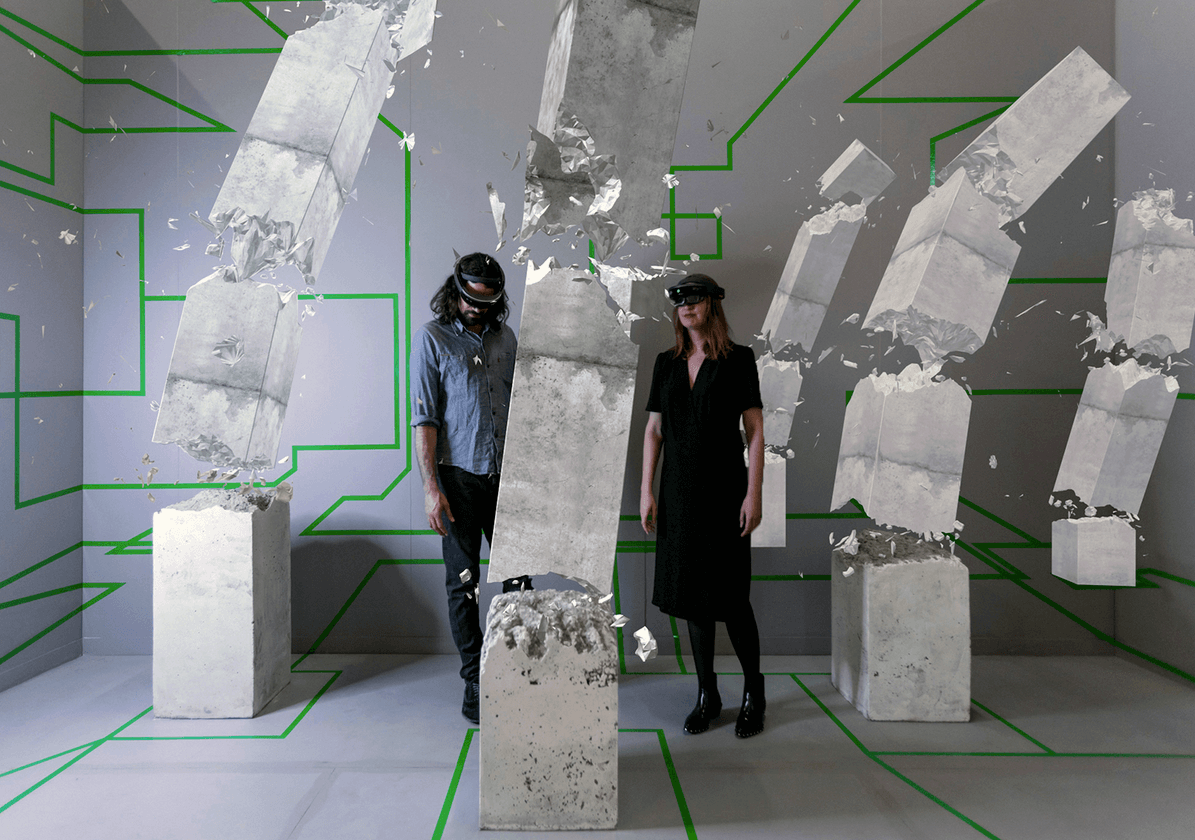
\includegraphics[width=.75\linewidth]{02-review/studiodrift.png}
    \captionsetup{justification=centering,margin=1.5cm}
    \caption{Composite AR view of Concrete Storm \citep[from][]{gordijn2017}}
\end{figure}\label{fig: concretestorm}

\subsection{Collaborative Expression}\label{sec: ar-arts-collaboration}
Another key aspect of the use of \gls{ar} as a medium in computational artworks is its ability to enable collaborative expression and construct shared perceptual spaces. For example, Listening Mirrors\footnote{\url{http://listeningmirrors.net/}}, an artwork by Chevalier and Kiefer, \citeyearpar{chevalier2018} is an \gls{ar} installation that engenders a collaborative and performative \gls{ar} sound environment. This environment is hybrid in nature; split between physical and virtual space. In the installation space, participants can interact with a audio augmented parabolic acoustic mirror. Their interactions are intertwined with a computationally mediated virtual sonic environment that they experience through bone conduction headphones. Additionally their vocalisations are mediated by a wearable microphone through the mirror. This invites collaborative expression through exploration of the shared sonic world.

Similarly, Eno and Chilvers explore collaborative ambient \gls{av} composition in their \gls{ar} adaptation of the popular app `Bloom', `Bloom: Space' \citep{eno2018}. In this installation, participants wear a Microsoft Hololens and use hand gestures to activate and manipulate generative \gls{av} elements. These elements can be experienced by other participants and thus create a shared perceptual and actionable space.

%*[ ]   fix figure
\begin{figure}[ht]
    \centering
    \captionsetup{justification=centering}
    \subcaptionbox{A participant interacting with the acoustic parabolic mirror in Listening Mirrors \citep[from][]{chevalier2019}\label{fig: collaborativeARt-listeningmirrors}}{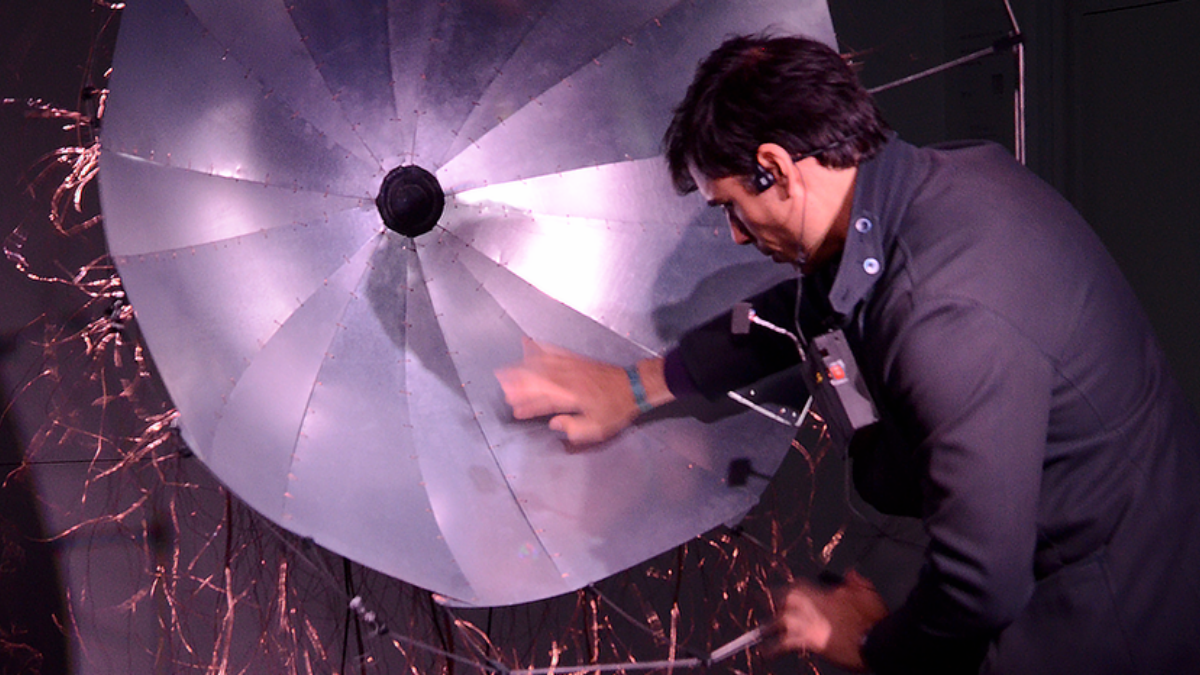
\includegraphics[width=0.45\linewidth]{02-review/chevalier18_1.png}}
    \hfill
    \subcaptionbox{Three immersed participants, creating sonic ARt in the Bloom: Space experience \citep[from][]{ray2018}\label{fig: collaborativeARt-bloom}}{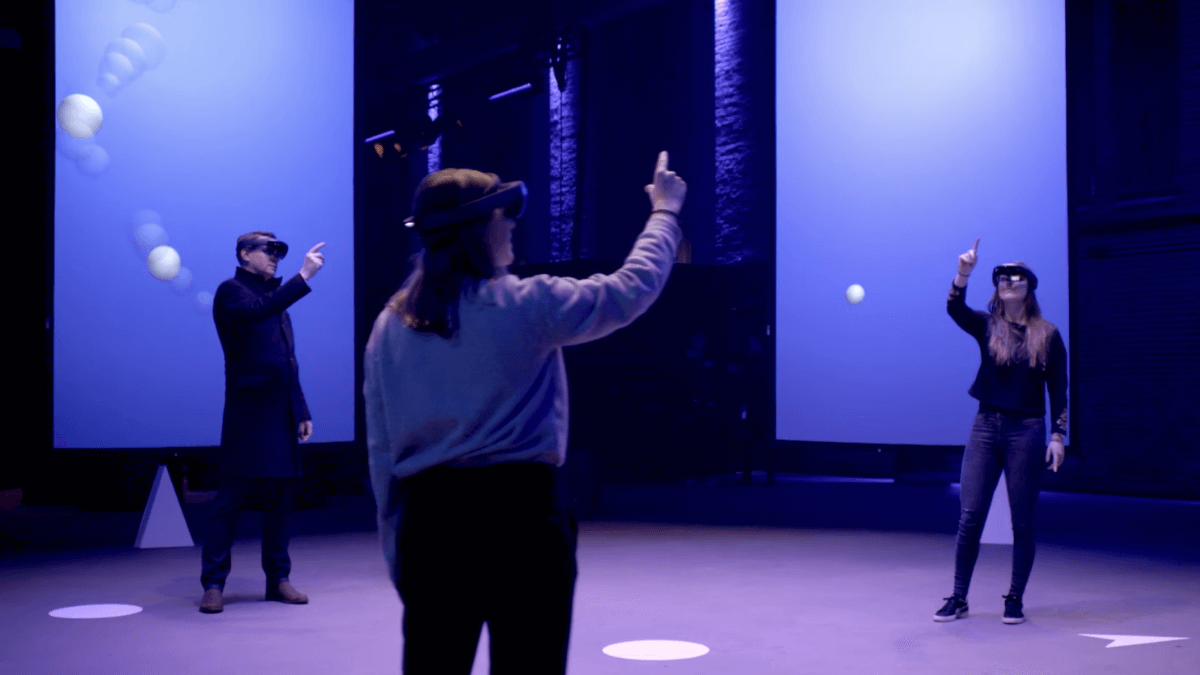
\includegraphics[width=0.45\linewidth]{02-review/bloom.png}}
    \caption{Collaborative Expression in AR}
    \label{fig: collaborativeARt}
\end{figure}

\subsection{Activism and Agency}\label{sec: ar-arts-activism}
Due to its ability to be an effective tool for collaborative expression, or perhaps because it creates a liminal hybridity that `questions the possession and control of a physical space' \citep{thiel2018}, \gls{ar} art has seen use in activism and collaborative political expression. Early pioneers such as the Manifest.AR group were able to create convincing and socially immersive \gls{ar} art using visual layering \citep{veenhof2010}. They did this through aligning the collaborative potential of \gls{ar} with political expression. By creating an app that overlaid visual art within the \gls{moma} through \gls{satnav}, they allowed participants to visit an exhibition in the museum that had not been organised by \gls{moma} themselves (\autoref{fig: activismARt-moma}). \gls{ar} thereby afforded these artists the ability to embed virtual art within an area considered private property, and also promote collective \gls{ar} agency, raising very early questions about `virtual trespass' with \gls{ar}. In a similar vein, `\#arOCCUPYWALLSTREET' (\#arOWS) was an arm of the Occupy Wall Street protests of 2011. Some 25 artists succeeded in overlaying the Wall Street area with `over 400 protest related augments', including audio overlays of protesters who were forbidden by police to enter the area. In this way, `\gls{ar} was able to overcome their surveillance, barricades, horses, and excessive police numbers' \citeyearpar{skwarek2018} and more easily provide the means to action to people unable to physically mobilise.

\begin{figure}
    \centering
    \captionsetup{justification=centering}
    \subcaptionbox{Manifest.AR MoMA Invasion \citep[from][]{veenhof2010}\label{fig: activismARt-moma}}{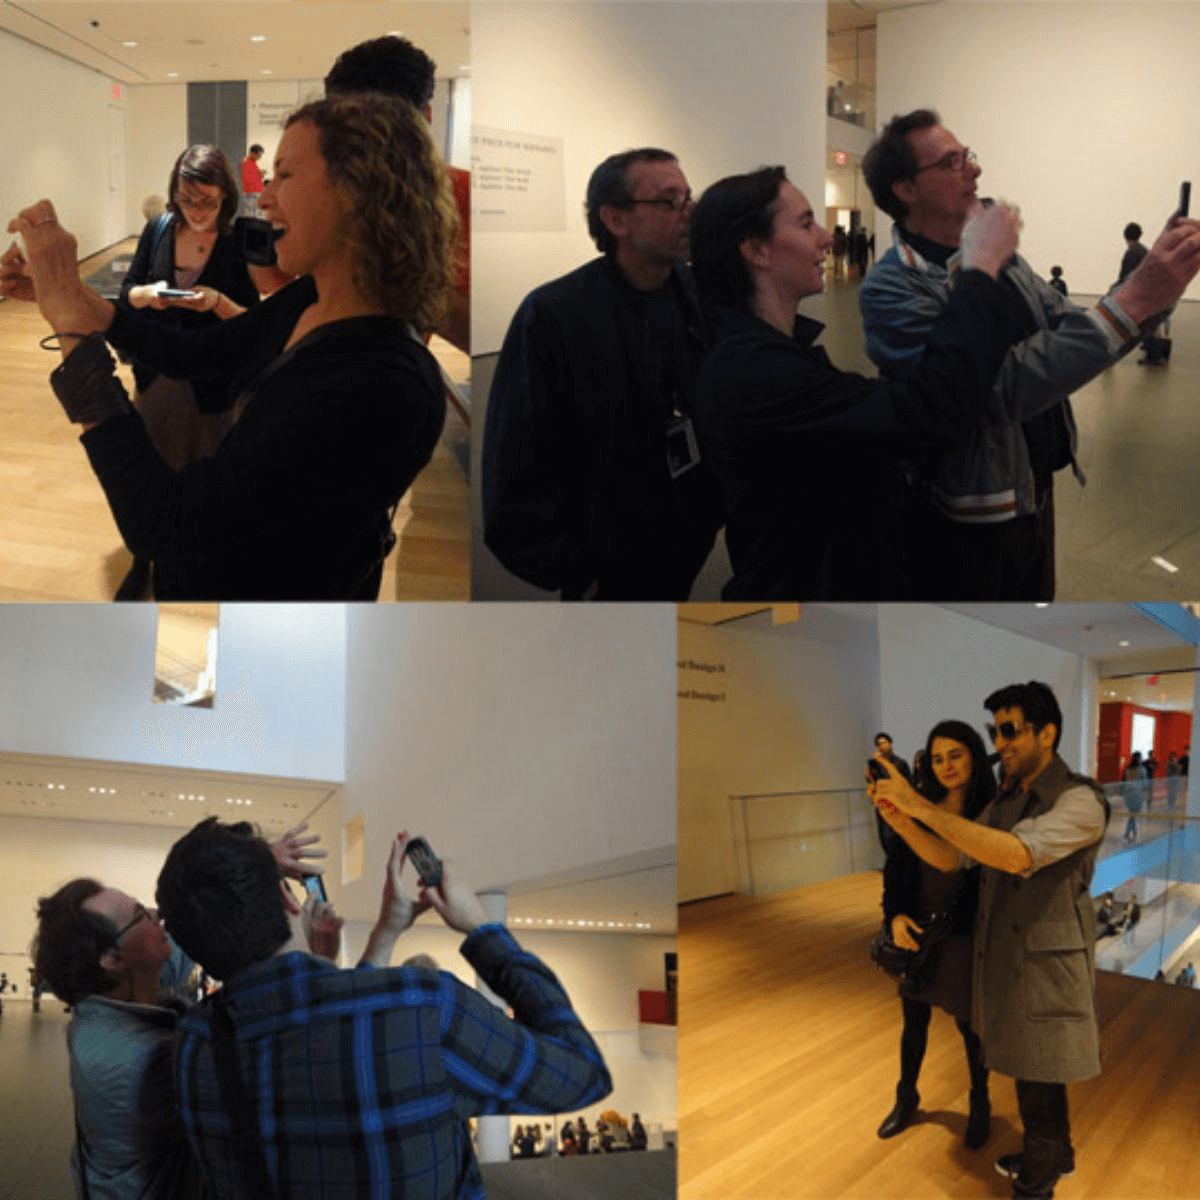
\includegraphics[width=0.45\linewidth]{02-review/moma.png}}
    \hfill
    \subcaptionbox{Invisible Istanbul \citep[from][]{thiel2011}\label{fig: activismARt-istanbul}}{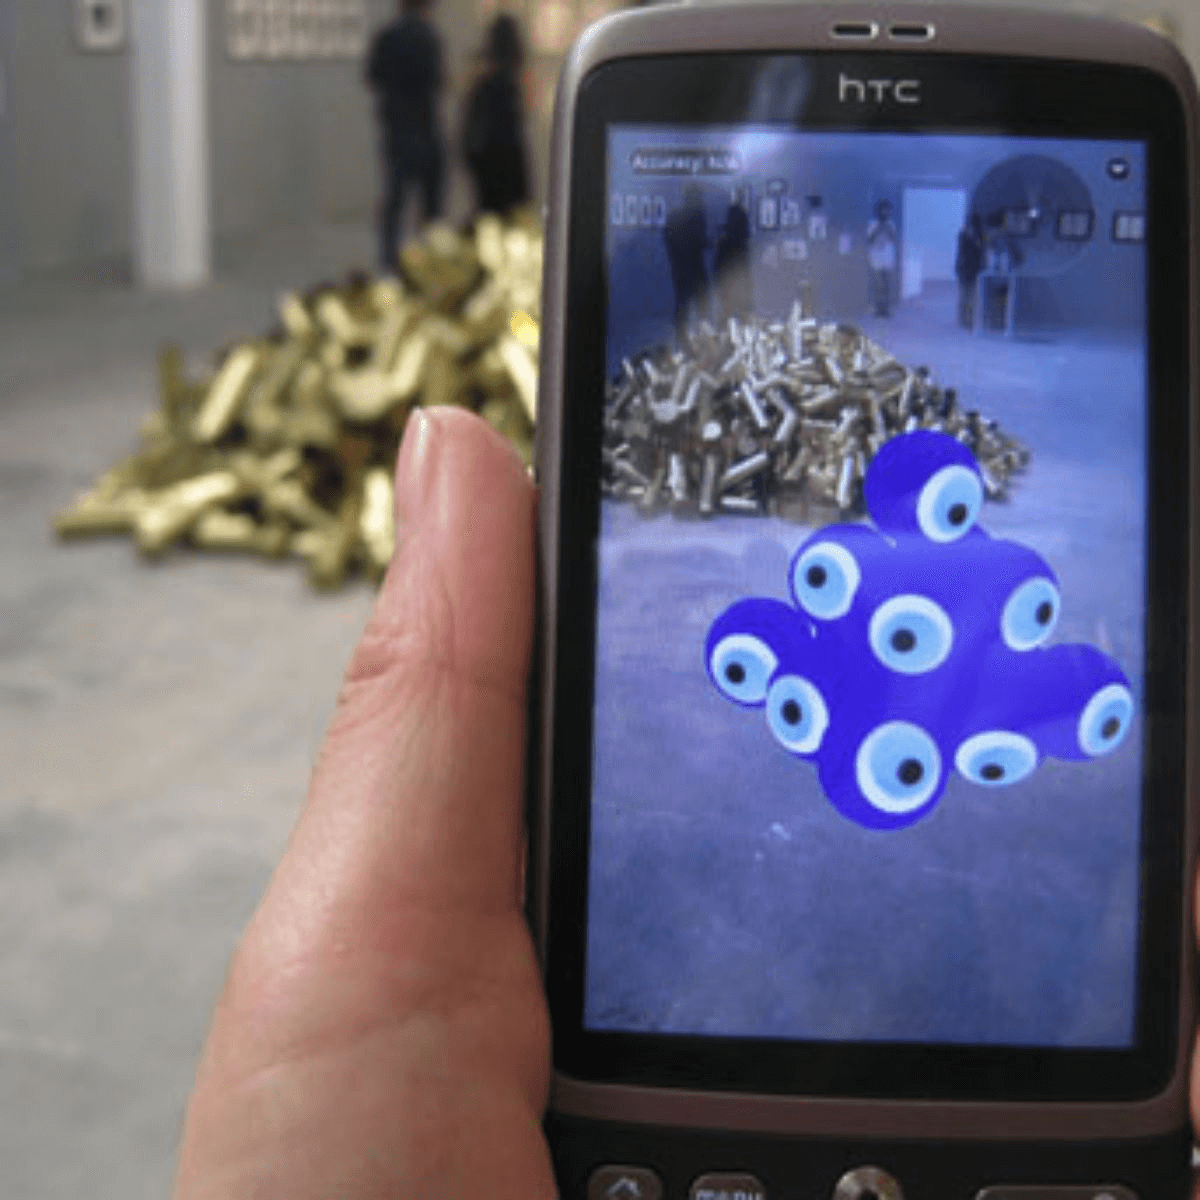
\includegraphics[width=0.45\linewidth]{02-review/thiel.png}}
    \caption{Activism through Interventionist ARt}
    \label{fig: activismARt}
\end{figure}

As well as its liminality between real and virtual space promoting otherwise dangerous collaborative expression, \gls{ar} has the power of rendering the invisible as seen, and due to this, it is a tool that has be used to shine light on social, economic, political and environmental injustices. Through its ability to change our perception of the real world through sensory augmentation, diminishment, hybridisation and extension, it has been used as a medium within the arts to `uncover' underlying mechanisms in our society. For example, Thiel and PATTU's (artists Cem Kozar and Işıl Ünal) 2011 work `Invisible Istanbul' aims to render the unseen urban dynamics of Istanbul visible through smartphone visual overlay and \gls{satnav}. They write: `Viewers become as photographers: the act of viewing or making a screenshot of the objects at a specific site and time reifies the virtual objects into artworks, revealing hidden forces within the city not visible to the naked eye.' \citeyearpar{thiel2011}. In PATTU's work, an \gls{ar} walking tour, different parts of the city are overlaid with symbolic information of past, present, and future uses of each area, highlighting tensions from military and commercial uses, and the effects this has on `contemporary urban space and the lives of its inhabitants' \citeyearpar{thiel2018}.



As summarised by Manifest.AR member Martin Skwarek puts it: `Alice has stepped through the looking glass [...] It is the job all future artists and activists to use this technology for the better, to bring people together, and uproot social injustice.' \citeyearpar{skwarek2018}

The next chapter delves into related research areas, including from the field of interactive music systems, where this thesis is situated, to further understand the \textit{materiality} afforded by \gls{ar} when used as a medium for creative expression specifically within sound art and music, the experience of \textit{embodiment} it has the potential of imparting on its immersants, and the hybrid real-virtual \textit{space} it co-constructs with them when in use.